\documentclass{project}
\usepackage[pdfauthor={N. W. Hardy},pdftitle={Software Engineering Group Project, LaTeX Document Example},pdftex]{hyperref}
\usepackage{graphicx}
\graphicspath{ {images/} }
\begin{document}
\title{Software Engineering Group Project}
\subtitle{Project Plan}
\author{Luke Jones}     
\shorttitle{LaTeX}
\version{1.0}
\status{Draft}
\date{2015-10-21}
\configref{SE-12-PM-01}
\maketitle
\tableofcontents
\newpage
\section{INTRODUCTION}
\subsection{Purpose of this Document}
The purpose of this document is to outline our project plan, to provide data on the time frame in which tasks are to completed and to provide information on risks associated with the project, and how their effects may be mitigated.
\subsection{Scope}
This document specifies the time frame in which we aim to begin and complete tasks and the team member(s) who will work on each task. This document also highlights any risks involved with the project with regard to delays, and includes instruction on how the effects of such delays can be mitigated.
\\[1\baselineskip]This document should be read and closely monitored by all project members. It is assumed that the reader is already familiar with QA document SE.QA.05b [1].
\subsection{Objectives}
The objectives of this document are as follows:
\begin {itemize}
	\item To provide group members with a prior knowledge of when major milestones will be targeted.
	\item Illustrate the optimal dates for the beginning and completion of tasks/subtasks.
	\item Outline group member(s) who will be responsible for the completion of each task.
	\item Identify parts of the plan with potential to cause delay, as well as any outside factors that could make task completion longer than necessary.
	\item Advise on course of action in the event of a delay occurring.
\end {itemize}	
\newpage
\section{GANTT CHART}
\begin{center}
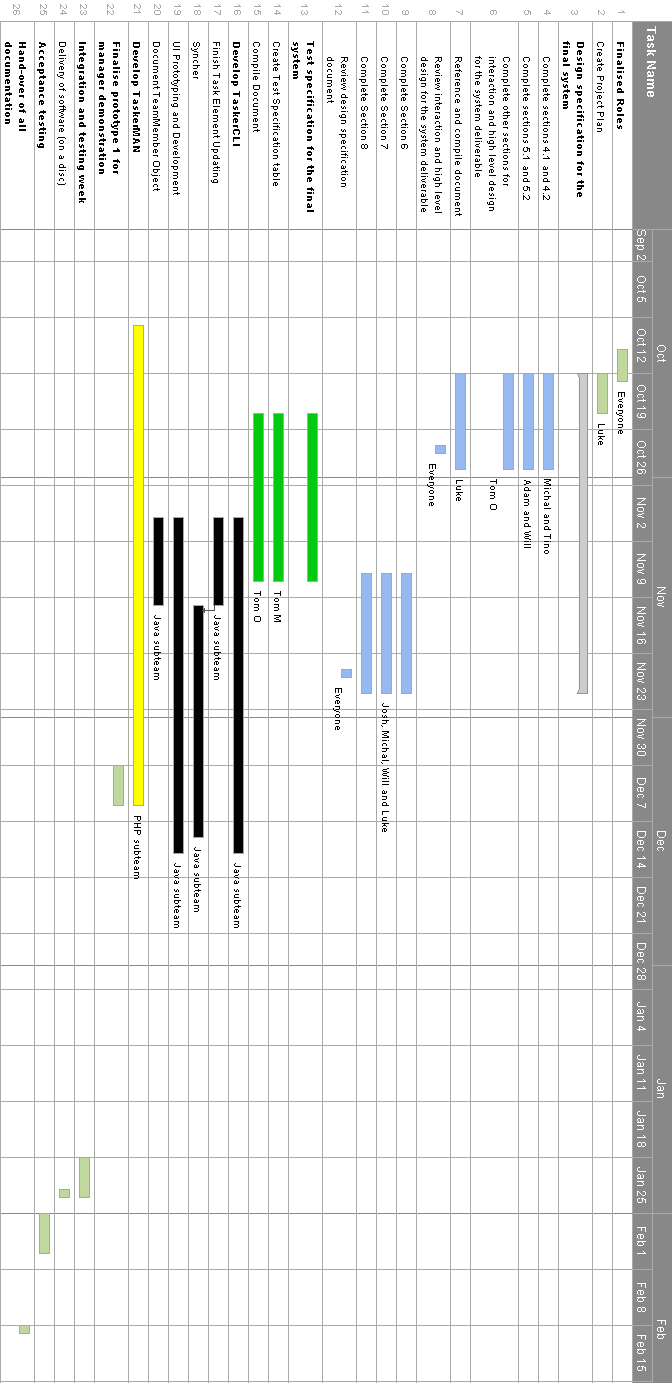
\includegraphics[width = 15cm, height = 26cm]{Ganttchart}
\end{center}
\newpage
\section{RISK ANALYSIS}
\begin{tabular}{ | p{3cm} | p{2cm} | p{2cm} | p{4cm} | p{4cm} |  }
  \hline
  \textbf{Risk} & \textbf{Probability of Risk 0-10} & \textbf{Risk Severity 0-10} & \textbf{Risk Description} & \textbf{Prevention Procedures} \\ \hline
Illness to member(s) of group & 5 & 3 & One or more members of the group are absent & Agile workload distribution, roles can be reallocated \\ \hline
Members not uploading to GitHub & 5 & 8 & A group member fails to upload their work to GitHub & Disciplinary action enforced by project leader \\ \hline
Unit testing not adequate & 4 & 9 & Testing falls below specifications & Enforce a testing team with multiple members with a wide skill range \\ \hline
Failure to understand brief requirements & 5 & 5 & Member of the group does not understand specific requirements & Have project leader seek clarification from superiors \\ \hline
University network malfunctioning & 2 & 7 & The university network is not working & Ensure group members have a backup of work they are currently working on \\ \hline
Members go over 80 hour limit & 5 & 10 & Group member goes over the allowed 80 hour limit & Reallocate work to different members of the group with less work time \\ \hline
Skill levels are not adequate & 5 & 6 & Members of the group have a low level of skill in specific areas
& Assign group members tasks according to their strengths \\ \hline
Members mis-understanding what is asked of them & 4 & 7 & Some members of the group may not understand what they have been assigned to do &  Have meeting minutes uploaded as soon as possible in clear detail\\
  \hline
\end{tabular}  
\addcontentsline{toc}{section}{REFERENCES}
\begin{thebibliography}{5}
\bibitem{se.qa.03} \emph{Software Engineering Group Projects}
General Documentation Standards.
C. J. Price, N. W. Hardy, B.P. Tiddeman SE.QA.03. 1.8 Release.
\end{thebibliography}
\addcontentsline{toc}{section}{DOCUMENT HISTORY}
\section*{DOCUMENT HISTORY}
\begin{tabular}{|l | l | l | l | l |}
\hline
Version & CCF No. & Date & Changes made to Document & Changed by \\
\hline
1.1 & N/A & 2015-20-11 & Updated Risk Analysis and Gantt Chart & Luke Jones\\
\hline
1.0 & N/A & 2015-10-22 & Initial creation & Luke Jones\\
\hline
\end{tabular}
\label{thelastpage}
\end{document}
\end{verbatim}
\label{fig:footer}
\end{figure}
\clearpage
\addcontentsline{toc}{section}{REFERENCES}
\begin{thebibliography}{5}
\bibitem{se.qa.03} \emph{Software Engineering Group Projects}
Project Plan Specification Standards.
B. P. Tiddeman, N. Hardy, SE.QA.05b. 1.3.
\end{thebibliography}
\addcontentsline{toc}{section}{DOCUMENT HISTORY}
\section*{DOCUMENT HISTORY}
\begin{tabular}{|l | l | l | l | l |}
\hline
Version & CCF No. & Date & Changes made to Document & Changed by \\
\hline
1.0 & N/A & 2015-10-22 & Initial creation & Luke Jones \\
\hline
\end{tabular}
\label{thelastpage}
\end{document}
